\documentclass[border=4pt]{standalone}
% Preámbulo común de las figuras. Cada figura es un documento standalone
% que se compila a SVG con scripts/build_figures.sh
\usepackage[utf8]{inputenc}
\usepackage{amsmath}
\usepackage{tikz}
\usepackage[american, siunitx]{circuitikz}
\usetikzlibrary{arrows.meta,calc,decorations.pathmorphing,patterns}
\tikzset{
  >={Stealth[length=2.2mm]},
  eje/.style={->, thin},
  hilo/.style={thick},
}
% Paleta común: tonos medios legibles sobre fondo claro
\definecolor{azul}{RGB}{31,94,168}
\definecolor{rojo}{RGB}{192,57,43}
\definecolor{verde}{RGB}{39,128,73}
\definecolor{naranja}{RGB}{211,120,30}
\definecolor{morado}{RGB}{125,60,152}

\begin{document}
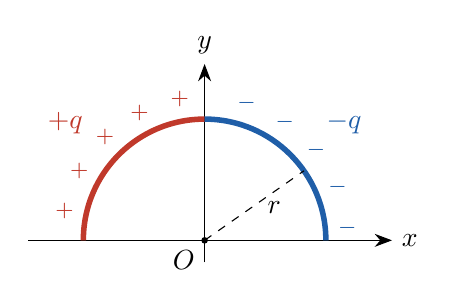
\begin{tikzpicture}[scale=1.4]
  \draw[eje] (-1.6,0) -- (1.7,0) node[right]{$x$};
  \draw[eje] (0,-0.2) -- (0,1.6) node[above]{$y$};
  \draw[line width=2pt, rojo] (180:1.1) arc (180:90:1.1);
  \draw[line width=2pt, azul] (90:1.1) arc (90:0:1.1);
  \foreach \a in {100,117,...,175} \node[text=rojo, font=\footnotesize] at (\a:1.3) {$+$};
  \foreach \a in {5,22,...,85} \node[text=azul, font=\footnotesize] at (\a:1.3) {$-$};
  \node[text=rojo] at (140:1.65) {$+q$};
  \node[text=azul] at (40:1.65) {$-q$};
  \draw[dashed] (0,0) -- node[pos=0.6, below right, inner sep=1pt]{$r$} (35:1.1);
  \fill (0,0) circle (0.03) node[below left]{$O$};
\end{tikzpicture}
\end{document}
